\documentclass{article}

\usepackage{amsmath}
\usepackage{graphicx}


\author{Alex Hiller}
\title{Extra Questions from Lab 2}

\begin{document}

\maketitle
\clearpage
\tableofcontents
\clearpage
\setlength{\parindent}{0cm}
\setlength{\parskip}{0.125cm}
\section{Balanced Load, Lagging Power Factor}
  \subsection{Question 5}  
  \textit{Compare your results in Table 2.1 and Table 2.5 and give your comments.} \\ \\
  \begin{centering}
  \begin{tabular}{|c|c|c|c|} \hline
    Quantity    & Table 2.1   & Measured in Lagging   & Difference (\%) \\ \hline
    $|V_{AN}|$  & 150.0 V     & 149.9 V               & 0.067     \\ \hline
    $|V_{AB}|$  & 259.8 V     & 262.8 V               & 1.142     \\ \hline
    $|V_{BC}|$  & 259.8 V     & 264.6 V               & 1.814     \\ \hline
    $|I_{A}|$   & 1.778 A     & 1.790 A               & 0.671     \\ \hline
    $|I_{B}|$   & 1.778 A     & 1.802 A               & 1.332     \\ \hline
    $|I_{C}|$   & 1.778 A     & 1.810 A               & 1.768     \\ \hline
    $P_{A}$     & 225 W       & 450 W                 & 50.00     \\ \hline
    $P_{C}$     & 225 W       & 235 W                 & 4.255     \\ \hline
    $P$         & 450 W       & 685 W                 & 34.31     \\ \hline
    $Q$         & 0 var       & 372.39 var            & $\infty$  \\ \hline
    $pf_A$      & 1 (?)       & 0.998                 & 0.200     \\ \hline
    $pf_C$      & 1 (?)       & 0.508                 & 96.85     \\ \hline
  \end{tabular} \\
  \end{centering}
  \noindent \\
  The voltages and currents were similar to those predicted before the lab. But parameters related to power were either poorly measured or poorly predicted (poorly predicted is more likely).\par
  Because the team assumed a positive phase sequence in experimentation, wattmeter measurements were made over the wrong phase. It is listed as $C$ phase, but because of the negative phase sequence of the bench, it is actually $B$ phase. Because of this, our two-wattmeter-method is very likely wrong and the power measurements would ideally be redone.

  % End Section 1
  \clearpage

\section{Balanced Load, Unity Power Factor}
  \subsection{Question 6}
  \textit{Compare your results in Table 2.2 and Table 2.6 and give your comments.} \\ \\
  \begin{centering}
  \begin{tabular}{|c|c|c|c|} \hline
    Quantity    & Table 2.2 & Measured in Unity  & Difference (\%)  \\ \hline
    $|I_{A}|$   & 1.5 A     & 1.581 A     &  5.122    \\ \hline
    $|I_{B}|$   & 1.5 A     & 1.586 A     &  5.422    \\ \hline
    $|I_{C}|$   & 1.5 A     & 1.599 A     &  6.191    \\ \hline
    $P_{A}$     & 337.5 W   & 341 W       &  1.026    \\ \hline
    $P_{C}$     & 337.5 W   & 363 W       &  7.025    \\ \hline
    $P$         & 675.0 W   & 704 W       &  4.119    \\ \hline
    $Q$         & 0 var     & -38.11 var  & $\infty$  \\ \hline
  \end{tabular} \\ 
  \end{centering} 
  \noindent \\ \\
  The currents $I_{B}$ and $I_{C}$ were not in the original Table 2.2 but assumedly they would also be of magnitude 1.5 Amperes in a balanced load with unity power factor. \par
  Measurements were very close to predicted, however measuring the percentage difference to a quantity that should be zero gives an inifinite difference, though only -38 var is a small enough amount to be due to imperfect elements used in the experiment (as opposed to the ideal ones used in the calculations).
  
  % End Section 2
  \clearpage


\section{Balanced Load, Leading Power Factor}
  \subsection{Nil}
    All questions were answered in the provided lab document.
  \clearpage

\section{Unbalanced Three-Wire Circuit}
   \subsection{Question 6}
   \textit{Use a graphical method for determining $V_{AO}$, $V_{BO}$ and $V_{CO}$ from $|V_{AO}|$, $|V_{BO}|$ and $|V_{CO}|$ and compare results with those of Table 2.4} \\ 

   \begin{figure}[!h]
     \centering
     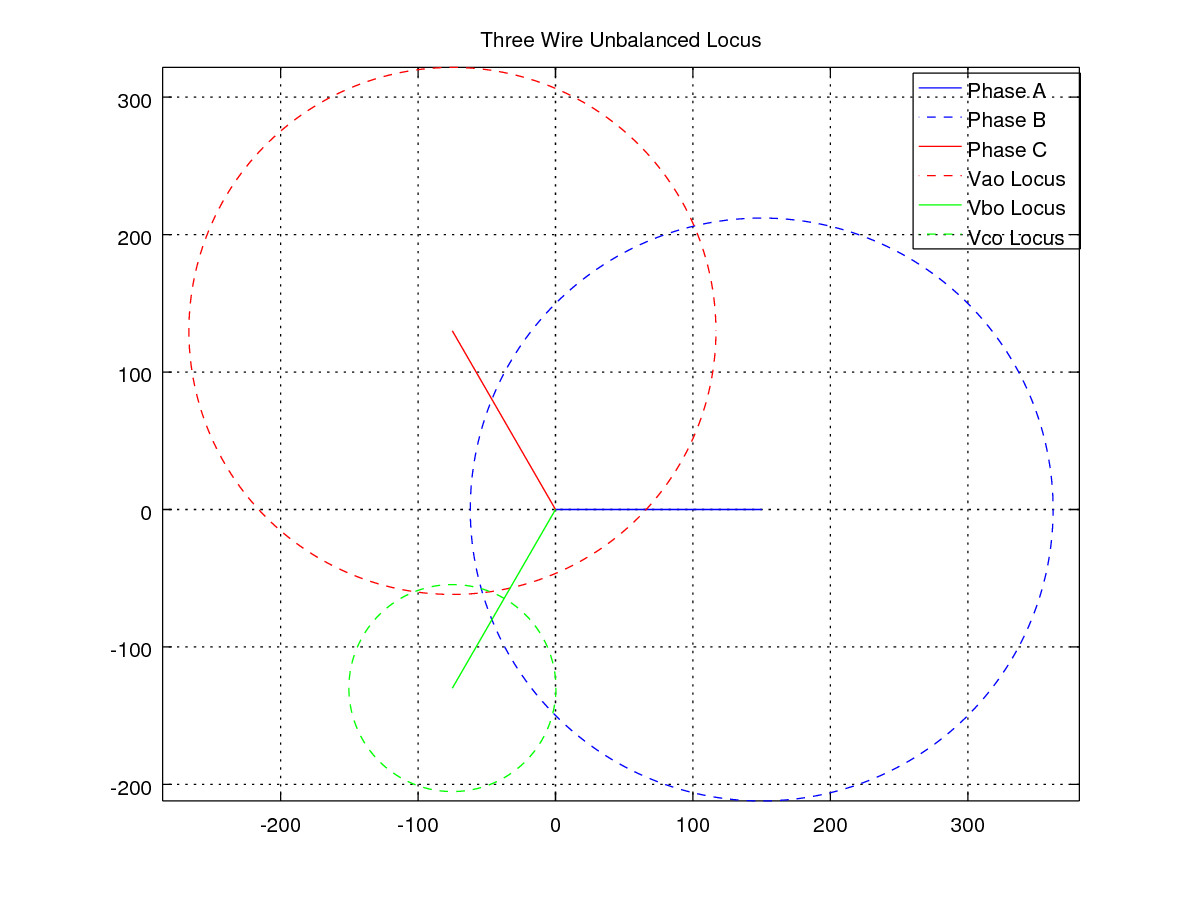
\includegraphics[width=0.8\textwidth]{Three_Phase_Unbalanced_Locus}
     \label{test}
   \end{figure}

   \begin{figure}[!h]
     \centering
     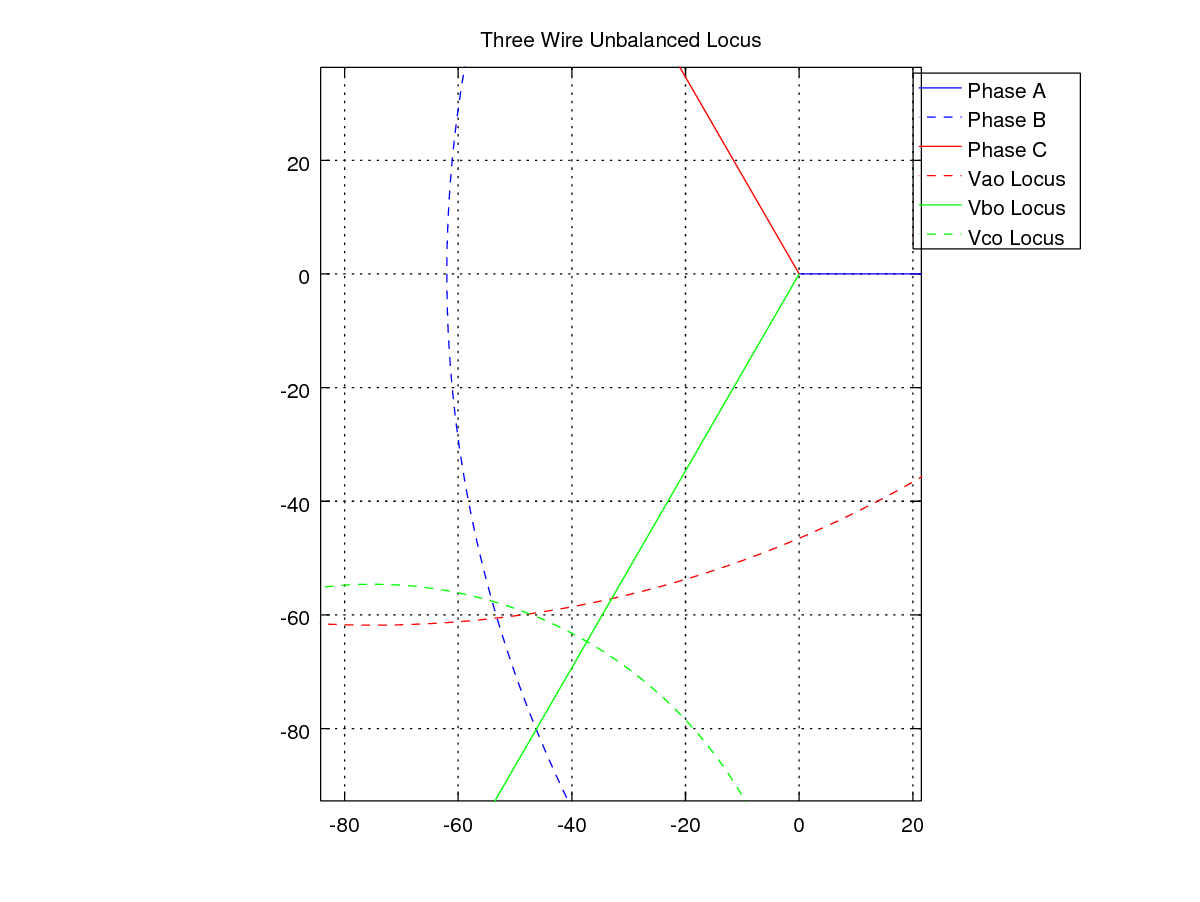
\includegraphics[width=0.8\textwidth]{von_determination}
     \label{test}
   \end{figure}

  \clearpage


  Looking at the loci closely, it can be seen that $V_{ON}$ can be approximated graphically by:
  
  $$
    \| V_{ON} \| = \sqrt{(-50)^2 + (-60)^2)} = 78.102 V
  $$
  $$
      \theta_{von} = 180 + \tan^{-1} \bigg(  \frac{-60}{-50}  \bigg) = 230.194^{o} V
  $$

  Graphical calculations:
  $$
    V_{AO}  = V_{AN} - V_{ON} = 150 \angle 0^o - 78.102 \angle230.194^o = 208.806\angle16.699^o
  $$

  $$
    V_{BO}  = V_{BN} - V_{ON} = 150 \angle 120^o - 78.102 \angle230.194^o = 191.541 \angle97.499^o  V
  $$

   $$
    V_{CO}  = V_{CN} - V_{ON} = 150 \angle 240^o - 78.102 \angle230.194^o = 74.2404 \angle-109.67^o V
  $$




   \begin{centering}
   \begin{tabular}{|c|c|c|c|} \hline
     Value   & Table 2.4                & Measured & Graphical \\ \hline
      V_{on} &  214.337 \angle127.134   & -  & 78.102 \angle230.194  \\ \hline
      V_{ao} &  327.502 \angle-31.4     & \| 212.7  \|  &   208.806\angle16.699^o  \\ \hline
      V_{bo} &  68 \angle-36.98         & \| 75.4  \| &  191.541 \angle97.499^o   \\ \hline
      V_{co} &  225 \angle 76.04        & \| 192.7  \|  &    74.2404 \angle-109.67^o  \\ \hline



   \end{tabular} \\
   \end{centering}
   \noindent \\ \\
    

   
   \subsection{Question 8}
   \textit{Give your comments and conclusions.}
   \par
   It would seem that the calculations were all done assuming positive phase sequence, but the bench itself instead had negative phase sequence. This can be deduced from the above table in the interchanged magnitudes of the $B$ and $C$ line. \par
  Besides this experimental mishap, it can be seen that an unbalanced three phase circuit can give widely varying circuit parameters. Even just slight change in parameters at the load can cause large variations between phases. 
   \clearpage

\section{Unbalanced Four-Wire Circuit}
  \subsection{Question 6}
  \textit{Use a phasor diagram to determine the expected value of $|I_{ON}|$ and compare this to the measured value.}
  \par
  \begin{centering}
  \begin{tabular}{|c|c|c|} \hline
    Value & Measured  (Absolute Value) & Graphical \\ \hline
    I_{O}   & 1.688  & Not Performed \\ \hline
    I_{AO}  & 0.904  & Not Performed \\ \hline
    I_{BO}  & 1.516  & Not Performed \\ \hline
    I_{CO}  & 1.528  & Not Performed \\ \hline
  \end{tabular} \\
  \end{centering}
  \noindent \\ \\
  
  
  \subsection{Question 8}
  \textit{Give your comments and conclusions.}
  \par
  
  \clearpage


\end{document}
